\documentclass{beamer}
\usepackage[style=ieee]{biblatex}
\usepackage[utf8]{inputenc}
\usepackage{listings}
\usepackage{pgffor}
\usepackage{minted}
\usepackage[prefix=]{xcolor-material}
\usetheme{seville}
\definecolor{buttonback}{HTML}{083444}
\makeatletter
\defbeamertemplate*{frametitle continuation}{only if multiple}{%
    \ifnum \numexpr\beamer@endpageofframe+1-\beamer@startpageofframe\relax > 1
        \textmd{(%
            \insertcontinuationcount/%
            \the\numexpr\beamer@endpageofframe+1-\beamer@startpageofframe%
        )}%
    \fi%
}
\makeatother

\setbeamercolor{button}{bg=buttonback,fg=Amber50!85!Grey}

\addbibresource{demo.bib}

\title{Simuler les feux de forêt}
\subtitle{Comment utiliser l'informatique pour réduire l'impact des feux de forêts en transformant le moins possible ces dernières ?}
\author{Victor Sarrazin}
\date{N° SCEI 14423}

\setbeamertemplate{footline}{%
  \raisebox{10pt}{% 
    \makebox[\paperwidth]{%
      \hfill\makebox[20pt]{%
        \large\textbf\insertframenumber 
      }
    }
  }
}

\begin{document}

\begin{frame}[plain]

    \titlepage

\end{frame}

\begin{frame}
    \frametitle{Introduction \hyperlink{jump}{\beamerbutton{ }} \hypertarget{1}{\beamerbutton{ }}}

    \begin{block}{Contexte}
        Les feux de forêt sont de plus en plus fréquents. L'informatique peut se révéler être un atout de taille pour contrer ces derniers
    \end{block}

    \begin{figure}
        \centering
        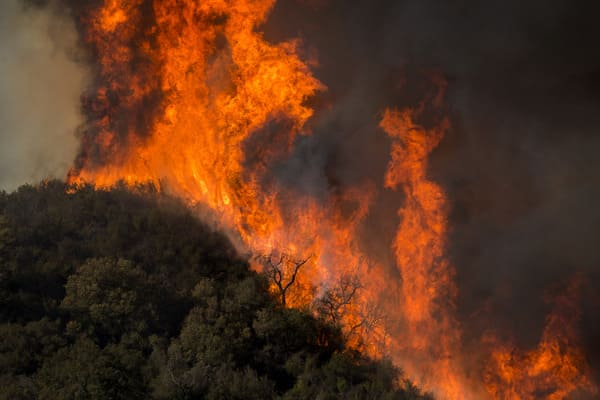
\includegraphics[width=0.5\linewidth]{pictures/intro.jpg}
        \caption{Feu de forêt à Malibu\footnote{National Geographic Education}}
        \label{fig:enter-label}
    \end{figure}
\end{frame}


\section{Un premier modèle de feux de forêt}
\section{Modèle d'Alexandridis pour les feux de forêt}
\section{Étude des transformations réalisables}

\begin{frame}{Sommaire \hyperlink{jump}{\beamerbutton{ }} \hypertarget{2}{\beamerbutton{ }}}
    \tableofcontents
\end{frame}

\begin{frame}{Un premier modèle de feux de forêt \hyperlink{jump}{\beamerbutton{ }} \hypertarget{3}{\beamerbutton{ }}}
    \begin{definition}{On définit un automate cellulaire (2D) avec :}
        \begin{itemize}
            \item Une grille
            \item Un état par case
            \item Un ensemble de règles de transitions entre les états
        \end{itemize}
    \end{definition}

    \visible<2-2>{\begin{figure}
        \centering
        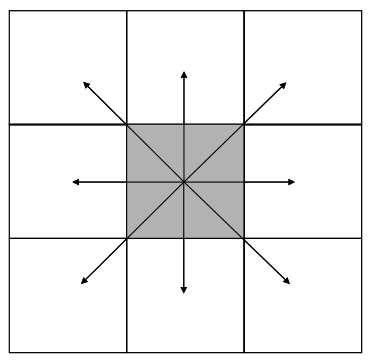
\includegraphics[width=0.25\linewidth]{pictures/moore.png}
        \caption{Voisinage de Moore\footnote{Science Direct}}
        \label{fig:enter-label}
    \end{figure}}
\end{frame}

\begin{frame}{Un premier modèle de feux de forêt \hyperlink{jump}{\beamerbutton{ }} \hypertarget{4}{\beamerbutton{ }}}
    \begin{definition}{On définit un automate cellulaire (2D) avec :}
        \begin{itemize}
            \item Une grille
            \item Un état par case
            \item Un ensemble de règles de transitions entre les états
        \end{itemize}
    \end{definition}

    \visible<2-2>{\begin{figure}
        \centering
        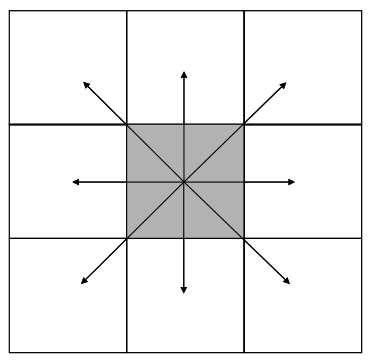
\includegraphics[width=0.25\linewidth]{pictures/moore.png}
        \caption{Voisinage de Moore\footnote{Science Direct}}
        \label{fig:enter-label}
    \end{figure}}
\end{frame}


\begin{frame}
    \frametitle{Navigateur \hypertarget{jump}{\beamerbutton{ }}}

    \hyperlink{1}{\beamerbutton{Diapo 1}} \\
    \hyperlink{2}{\beamerbutton{Diapo 2}}
\end{frame}

% \begin{frame}[
% t, % align text from top
% allowframebreaks, % allow brake frames
% fragile % allow verb content
% ]{main.c}
%     \scriptsize
%     \inputminted[breaklines,breakanywhere,fontsize=\tiny,
%     tabsize=2]{c}{code/main.c}
% \end{frame}
% \begin{frame}[
% t, % align text from top
% allowframebreaks, % allow brake frames
% fragile % allow verb content
% ]{misc.c}
%     \scriptsize
%     \inputminted[breaklines,breakanywhere,fontsize=\tiny,
%     tabsize=2]{c}{code/misc.c}
% \end{frame}
% \begin{frame}[
% t, % align text from top
% allowframebreaks, % allow brake frames
% fragile % allow verb content
% ]{grid.c}
%     \scriptsize
%     \inputminted[breaklines,breakanywhere,fontsize=\tiny,
%     tabsize=2]{c}{code/grid.c}
% \end{frame}
% \begin{frame}[
% t, % align text from top
% allowframebreaks, % allow brake frames
% fragile % allow verb content
% ]{typings.c}
%     \scriptsize
%     \inputminted[breaklines,breakanywhere,fontsize=\tiny,
%     tabsize=2]{c}{code/typings.c}
% \end{frame}
% \begin{frame}[
% t, % align text from top
% allowframebreaks, % allow brake frames
% fragile % allow verb content
% ]{draw.c}
%     \scriptsize
%     \inputminted[breaklines,breakanywhere,fontsize=\tiny,
%     tabsize=2]{c}{code/draw.c}
% \end{frame}

\end{document}
